% interactcadsample.tex
% v1.03 - April 2017

\documentclass[]{interact}

\usepackage{epstopdf}% To incorporate .eps illustrations using PDFLaTeX, etc.
\usepackage{subfigure}% Support for small, `sub' figures and tables
%\usepackage[nolists,tablesfirst]{endfloat}% To `separate' figures and tables from text if required

\usepackage{natbib}% Citation support using natbib.sty
\bibpunct[, ]{(}{)}{;}{a}{}{,}% Citation support using natbib.sty
\renewcommand\bibfont{\fontsize{10}{12}\selectfont}% Bibliography support using natbib.sty

\theoremstyle{plain}% Theorem-like structures provided by amsthm.sty
\newtheorem{theorem}{Theorem}[section]
\newtheorem{lemma}[theorem]{Lemma}
\newtheorem{corollary}[theorem]{Corollary}
\newtheorem{proposition}[theorem]{Proposition}

\theoremstyle{definition}
\newtheorem{definition}[theorem]{Definition}
\newtheorem{example}[theorem]{Example}

\theoremstyle{remark}
\newtheorem{remark}{Remark}
\newtheorem{notation}{Notation}

% see https://stackoverflow.com/a/47122900

% Pandoc citation processing

\usepackage{hyperref}
\usepackage[utf8]{inputenc}
\def\tightlist{}
\newcommand*{\Perm}[2]{{}^{#1}\!P_{#2}}%
\usepackage{booktabs}
\usepackage{longtable}
\usepackage{array}
\usepackage{multirow}
\usepackage{wrapfig}
\usepackage{float}
\usepackage{colortbl}
\usepackage{pdflscape}
\usepackage{tabu}
\usepackage{threeparttable}
\usepackage{threeparttablex}
\usepackage[normalem]{ulem}
\usepackage{makecell}
\usepackage{xcolor}

\begin{document}

\articletype{ARTICLE TEMPLATE}

\title{Why aren't significance tests commonly used for linear regression
diagnostics?}


\author{\name{Weihao Li$^{a}$, Dianne Cook$^{a}$, Emi
Tanaka$^{a}$, Susan VanderPlas$^{b}$}
\affil{$^{a}$Department of Econometrics and Business Statistics, Monash
University, Clayton, VIC, Australia; $^{b}$Department of Statistics,
University of Nebraska, Lincoln, Nebraska, USA}
}

\thanks{CONTACT Weihao
Li. Email: \href{mailto:weihao.li@monash.edu}{\nolinkurl{weihao.li@monash.edu}}, Dianne
Cook. Email: \href{mailto:dicook@monash.edu}{\nolinkurl{dicook@monash.edu}}, Emi
Tanaka. Email: \href{mailto:emi.tanaka@monash.edu}{\nolinkurl{emi.tanaka@monash.edu}}, Susan
VanderPlas. Email: \href{mailto:susan.vanderplas@unl.edu}{\nolinkurl{susan.vanderplas@unl.edu}}}

\maketitle

\begin{abstract}
Abstract to fill.
\end{abstract}

\begin{keywords}
data visualization; visual inference; hypothesis testing; residual
plots;
\end{keywords}

\hypertarget{introduction}{%
\section{Introduction}\label{introduction}}

\begin{quote}
\emph{``Since all models are wrong the scientist must be alert to what
is importantly wrong.''} \citep{box1976science}
\end{quote}

Diagnosing a model is the key to determining whether there is anything
importantly wrong. For linear regression analysis, it is typical to
interrogate the residuals. Residuals summarise what is not captured by
the model, and thus provide the capacity to identify what might be
wrong. There are many ways that residuals could be assessed.

Residuals might be plotted, as a histogram or quantile-quantile plot to
examine the distribution. Using the classical normal linear regression
model as an example, if the distribution is symmetric and unimodal, it
is well-behaved. But if the distribution is skewed, bimodal, multimodal,
or contains outliers, there is cause for concern. The distribution could
also be inspected by conducting a goodness of fit test, such as the
Shapiro-Wilk Normality test \citep{shapiro1965analysis}.

Plotting the residuals against predicted values and each of the
explanatory variables on a scatter plot is a recommend way to scrutinize
their relationships. If there is any visually discoverable patterns, the
model is potentially misspecified. However, it is a very difficult task
for a human judge, though to make a decision that there's nothing there.
It is especially common, particularly among new data analysts to report
patterns when an experienced data analyst might quickly conclude that
there are none. Generally, one looks for departures from nothingness
like non-linear dependency or heteroskedasticity. It is also possible to
conduct hypothesis tests for non-linear dependence
\citep{ramsey_tests_1969}, and use a Breusch-Pagan test
\citep{breusch_simple_1979} for heteroskedasticity.

There is an abundance of literature describing appropriate diagnostic
methods for linear regression: \citet{draper1998applied},
\citet{montgomery1982introduction}, \citet{belsley_regression_1980},
\citet{cook_applied_1999} and \citet{cook1982residuals}. The diligent
reader of these sage writings will also notice sentences that express
sentiments like \emph{based on their experience, statistical tests are
not widely used in regression diagnostics. The same or even larger
amount of information can be provided by diagnostic plots than the
corresponding tests in most empirical studies.} There is a common
guidance by experts that plots are the best for diagnosing model fits.

This is curious, and investigating why this might be common advice is
the subject of this paper. The paper is structured as follows. The next
background section describes the the types of departures that one
expects to detect, and describes a formal process for reading residual
plots, called visual inference, that can avoid the concerns about
subjectiveness of human readers. Section \ref{experimental-design}
describes the experimental setup to enable a comparison between decision
made by formal hypothesis testing, and how humans would read diagnostic
plots. The results are reported in Section \ref{results}. We finish with
a discussion on future work, in particular how the responsibility for
residual plot reading might be passed on to computer vision.

\hypertarget{background}{%
\section{Background}\label{background}}

\hypertarget{departures-from-good-residual-plots}{%
\subsection{Departures from good residual
plots}\label{departures-from-good-residual-plots}}

(This section discusses the visual patterns data analysts expect to see
and their implications.)

\begin{figure}
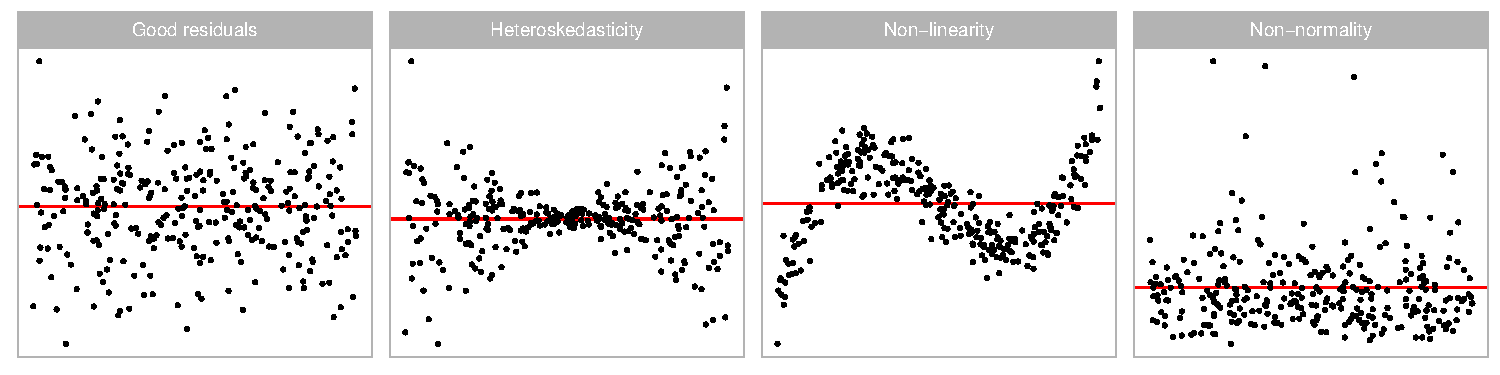
\includegraphics[width=1\linewidth]{paper_comparison_files/figure-latex/residual-plot-common-departures-1} \caption{Example fitted vs residual plots: (A) classically good looking residuals, (B) non-linear pattern indicates that the model has not captured a non-linear association, (C) heteroskedasticity indicating that variance around the fitted model is not uniform, and (D) non-normality where the residual distribution is not symmetric around 0. The latter pattern might best be assessed using a univariate plot of the residuals, but patterns B and C need to be assessed using a residual vs fitted plot.}\label{fig:residual-plot-common-departures}
\end{figure}

Graphical summaries in which residuals are plotted against fitted values
or other functions of the predictor variables that are approximately
orthogonal to residuals are referred to as standard residual plots in
\citet{cook1982residuals}. As shown in Figure
\ref{fig:residual-plot-common-departures}, the top-left panel is a good
residual plot with residuals evenly distributed at both sides of the
horizontal zero line showing no noticeable patterns. There are various
types of departures from a good residual plot.

Non-linearity, heterskedasticity and non-normality are perhaps the three
mostly commonly checked departures. Non-linearity is a type of model
misspecification caused by failing to include higher order terms of the
regressors in the regression equation. Any non-linear functional form of
residuals on fitted values presented in the residual plot could be
considered as an indicative of non-linearity. An example residual plot
containing visual pattern of non-linearity is given at the top-right of
Figure {[}ref here{]}. One can clearly observe the ``S-shape'' from the
residual plot as the cubic term is not captured by the misspecified
model. Heterskedasticity refers to the presence of nonconst error
variance in a regression model. It is mostly due to the strict but false
assumptions on the variance-covariance matrix of the error term. The
usual pattern of heterskedasticity on a residual plot is the
inconsistent spread of the residuals at different x values. Visually, it
sometimes results in the so-called ``butterfly'' shape as shown in the
bottom-left panel of Figure \ref{fig:residual-plot-common-departures},
or the ``left-triangle'' and ``right-triganle'' shape where the smallest
variance occurs at the edges of the x-axis. Compared to non-linearity
and heterskedasticity, non-normality is usually harder to be detected
from a residual plot since scatter plot is not excel in revealing
marginal distribution. A favourable graphical summarise for this task is
the quantile-quantile plot. However, for a consistent comparison in the
later part of this paper, residual plot will be the focus. Besides, it
is important to note that not all regression models assume normality for
the error term, but a certain amount do including the classical normal
linear regression model. In the case that the normality assumption is
violated, it is expected to observe data points that do not centralize
around the horizontal zero line and unevenly distribute at both sides of
the zero line. For example, given a skewed error distribution, fewer
data points and more outliers are on one side of the zero line as shown
at the bottom-right of Figure \ref{fig:residual-plot-common-departures}.

\hypertarget{conventionally-testing-for-departures}{%
\subsection{Conventionally testing for
departures}\label{conventionally-testing-for-departures}}

(This section discusses the tests that will be used in the analysis and
shows the results for the residual plots displayed in the previous
section.)

Other than checking diagnostic plots, analysts may perform formal
hypothesis testing for detecting model defects. Depending on the
alternative hypothesis that is focused on, a variety of tests can be
applied. For example, the presence of heteroskedasticity can usually be
tested by applying the White test
\citep{white_heteroskedasticity-consistent_1980} or the Breusch-Pagan
test \citep{breusch_simple_1979}, which are both derived from the
Lagrange multiplier test \citep{silvey1959lagrangian} principle that
relies on the asymptotic properties of the null distribution. For
testing non-linearity, one may apply the F-test as a model structural
test to examine the significance of specific polynomial and non-linear
forms of the regressors, or the significance of proxy variables as in
the Ramsey Regression Equation Specification Error Test (RESET)
\citep{ramsey_tests_1969}. And for testing normality, the Shapiro--Wilk
test {[}ref here{]} is perhaps the most widely used test included by
many of the statistical softwares. Another choice will be the
Jarque--Bera test {[}ref here{]} which directly checks if the sample
skewness and kurtosis match a normal distribution.

Example residual plots given in Figure
\ref{fig:residual-plot-common-departures} are examined by the
corresponding model structural test, Breusch-Pagan test and
Shapiro--Wilk test as shown in Table
\ref{tab:example-residual-plot-table}. In the example, both the
Breusch-Pagan test and the Shapiro--Wilk test rejects the null
hypothesis for departures that they do not intend to examine. As
discussed in \citet{cook1982residuals}, most residual-based tests for a
particular type of departure from model assumptions are sensitive to
other types of departures. It is likely the null hypothesis is correctly
rejected but for the wrong reason, which is known as the ``Type III
error''. Additionally, outliers will often incorrectly trigger the
rejection of the null hypothesis despite the residuals are well-behaved
\citep{cook_applied_1999}. This can be largely avoided in diagnostic
plots as experienced analysts can evaluate the acceptability of
assumptions flexibly, even in the presence of outliers.

\begin{table}

\caption{\label{tab:example-residual-plot-table}Statistical significance testing for departures from good residuals for plots in Figure \ref{fig:residual-plot-common-departures}. Shown are the $p$-values calculated for the conventional Model structural, the Breusch-Pagan and the Shapiro–Wilk tests. The good residual plot (A) is judged a good residual plot, as expected, by all tests. The non-linearity (B) is detected by all tests, as might be expected given the extreme structure.}
\centering
\begin{tabular}[t]{llrrr}
\toprule
Plot & Departures & Model structural & Breusch-Pagan & Shapiro–Wilk\\
\midrule
A & None & 0.434 & 0.133 & 0.728\\
B & Non-linearity & \em{0.000} & \em{0.000} & \em{0.039}\\
C & Heteroskedasticity & 0.378 & \em{0.000} & \em{0.000}\\
D & Non-normality & 0.667 & 0.736 & \em{0.000}\\
\bottomrule
\end{tabular}
\end{table}

\hypertarget{visual-testing-for-departures}{%
\subsection{Visual testing for
departures}\label{visual-testing-for-departures}}

(This section introduces the lineup protocol, and briefly discusses the
method for sampling null data, calculating the p-value and estimating
power.)

\hypertarget{lineup-protocol}{%
\subsubsection{Lineup protocol}\label{lineup-protocol}}

Unlike hypothesis testing built upon rigorous statistical procedures,
reading diagnostic plots relies on graphical perception - human's
ability to interpret and decode the information embedded in the graph
\citep{cleveland_graphical_1984}, which is to some extent subjective and
indecisive. Further, visual discovery suffers from its unsecured and
unconfirmed nature where the degree of the presence of the visual
features typically can not be measured quantitatively and objectively,
which may lead to over or under-interpretations of the data. One such
example is finding an over-interpretation of the separation between gene
groups in a two-dimensional projection from a linear discriminant
analysis when in fact there are no differences in the expression levels
between the gene groups and separation is not an uncommon occurrence
\citep{roy_chowdhury_using_2015}.

Visual inference was first introduced in a 1999 Joint Statistical
Meetings (JSM) talk with the title ``Inference for Data Visualization''
by \citet{buja_inference_1999} as an idea to address the issue of valid
inference for visual discoveries of data plots
\citep{gelman_exploratory_2004}. Later, \citet{buja_statistical_2009}
proposed the lineup protocol as a visual test inspired by the ``police
lineup'' or ``identity parade'' which is the act of asking the
eyewitness to identify criminal suspect from a group of irrelevant
people. The protocol consists of \(m\) randomly placed plots, where one
plot is the actual data plot, and the remaining \(m - 1\) plots have the
identical graphical production as the data plot except the data has been
replaced with data consistent with the null hypothesis. Then, an
observer who have not seen the actual data plot will be asked to point
out the most different plot from the lineup. Under the null hypothesis,
it is expected that the actual data plot would have no distinguishable
difference with the null plots, and the probability of the observer
correctly picks the actual data plot is \(1/m\). If we reject the null
hypothesis as the observer correctly picks the actual data plot, then
the Type I error of this test is \(1/m\).

\begin{figure}
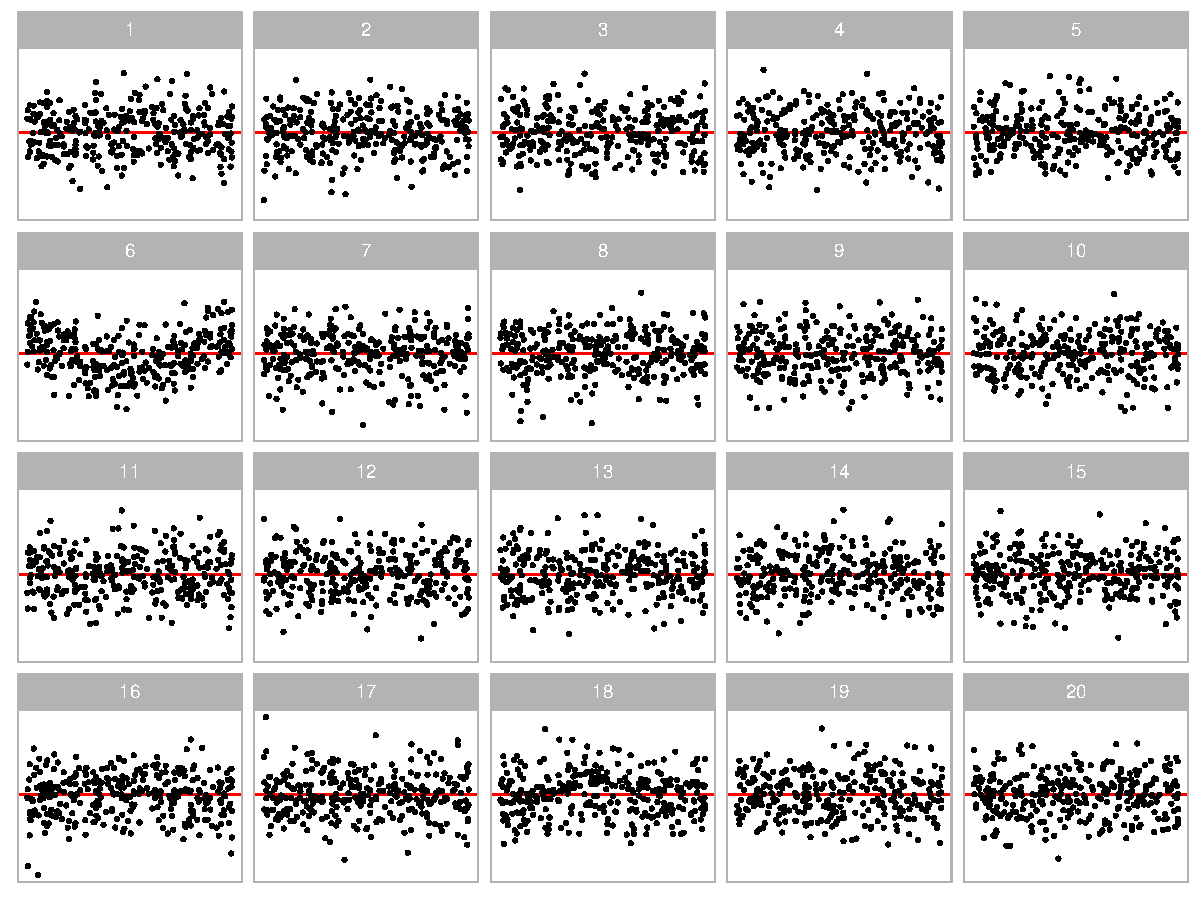
\includegraphics[width=1\linewidth]{paper_comparison_files/figure-latex/first-example-lineup-1} \caption{Visual testing is conducted using a lineup, as in the example here. The residual plot computed from the observed data (plot 11, exhibiting non-linearity) is embedded among 19 null plots, where the residuals were simulated from a standard error model. Computing the $p$-value requires that the lineup be examined by a number of human judges, each asked to select the most different plot. A small $p$-value would result from a substantial number selecting plot 11.}\label{fig:first-example-lineup}
\end{figure}

Figure \ref{fig:first-example-lineup} is an example of a lineup
protocol. If the actual data plot at position 11 is identifiable, then
it is evidence for the rejection of the null hypothesis that the
regression model is correctly specified. In fact, the actual residual
plot is obtained from a misspecified regression model with non-linearity
issue.

The effectiveness of lineup protocol has already been validated by
\citet{majumder_validation_2013} under relatively simple classical
normal linear regression model settings with only one or two regressors.
Their results suggest visual test is capable of testing the significance
of a single regressor with a similar power as a t-test, though they
expressed that in general it is unnecessary to use visual inference if
there exists a conventional test and they didn't expect the visual test
to perform equally well as the conventional test. In their third
experiment, where there does not exist a proper conventional test,
visual test outperforms the conventional test for a large margin. This
is encouraging as it promotes the use of visual inference in border
field of data science where there are no existing statistical testing
procedures. In fact, lineup protocol has been integrated successfully
into diagnostic tools of hierarchical linear models
\citep{loy2013diagnostic}.

\hypertarget{sampling-from-the-null-distribution}{%
\subsubsection{Sampling from the null
distribution}\label{sampling-from-the-null-distribution}}

Data used in the \(m - 1\) null plots need to be simulated. In the
context of regression diagnostics, sampling data from \(H_0\) is
equivalent to sampling data from the assumed model. As
\citet{buja_statistical_2009} suggested, \(H_0\) is usually composited
by a collection of distributions controlled by nuisance parameters.
Since regression models can have various forms, there is no general
solution to this problem, but it sometimes can be reduced to so called
``reference distribution'' by applying one of the three methods: (i)
sampling from a conditional distribution given a minimal sufficient
statistic under \(H_0\), (ii) parametric bootstrap sampling with
nuisance parameters estimated under \(H_0\), and (iii) Bayesian
posterior predictive sampling. The conditional distribution given a
minimal sufficient statistic is the best justified reference
distribution among the three \citep{buja_statistical_2009}. Essentially,
null residuals can be simulated by regressing \(N\) i.i.d standard
normal random draws on the regressors, then rescaling it by the ratio of
residual sum of square in two regressions.

\hypertarget{calculating-p-values}{%
\subsubsection{\texorpdfstring{Calculating
\(p\)-values}{Calculating p-values}}\label{calculating-p-values}}

Further, a visual test can involve \(K\) independent observers. Let
\(D_i = \{0,1\}\) be a binomial random variable denoting whether subject
\(i\) correctly detecting the actual data plot, and
\(X = \sum_{i=1}^{K}X_i\) be the number of observers correctly picking
the actual data plot. Then, by imposing a relatively strong assumption
on the visual test that all \(K\) evaluations are fully independent,
under the null hypothesis, \(X \sim \mathrm{Binom}_{K,1/m}\). Therefore,
the \(p\)-value of a lineup of size \(m\) evaluated by \(K\) observer is
given as \(P(X \geq x) = 1 - F(x) + f(x)\), where \(F(.)\) is the
cumulative distribution function, \(f(.)\) is the probability mass
function and \(x\) is the realization of number of observers correctly
picking the actual data plot \citep{majumder_validation_2013}.

As pointed out by \citet{vanderplas2021statistical}, the binomial model
doesn't take into account the possible dependencies in the visual test
due to repeated evaluations of the same lineup. And it is inapplicable
to visual test where subjects are asked to select one or more ``most
different'' plots from the lineup. They summarized three common
scenarios in visual inference: (1) \(K\) different lineups are shown to
\(K\) subjects, (2) \(K\) lineups with different null plots but the same
actual data plot are shown to \(K\) subjects, and (3) the same lineup is
shown to \(K\) subjects. Out of these three scenarios, Scenario 3 is the
most common in previous studies as it puts the least constraints on the
experimental design. For Scenario 3, \citet{vanderplas2021statistical}
modelled the probability of a plot \(i\) being selected from a lineup as
\(\theta_i\), where \(\theta_i \sim Dirichlet(\alpha)\) for
\(i=1,...,m\) and \(\alpha > 0\). And defined \(c_i\) to be the number
of times plot \(i\) being selected in \(K\) evaluations. In case subject
\(j\) makes multiple selections, \(1/s_j\) will be added to \(c_i\)
instead of one, where \(s_j\) is the number of plots subject \(j\)
selected for \(j=1,...K\). This ensured \(\sum_{i}c_i=K\). Since we are
only interested in the selections of the actual data plot \(i\), the
marginal model can be simplified to a beta-binomial model and thus the
visual p-value is given as

\begin{equation} \label{eq:pvalue-beta-binomial}
P(C \geq c_i) = \sum_{x=c_i}^{K}\frac{\Gamma(K + 1)}{\Gamma(x + 1)\Gamma(K - x + 1)}\frac{B(x + \alpha, K - x + (m - 1)\alpha)}{B(\alpha, (m-1)\alpha)},
\end{equation}

where \(B(.)\) is the beta function defined as

\begin{equation} \label{eq:betafunction}
B(a, b) = \int_{0}^{1}t^{\alpha - 1}(1-t)^{b-1}dt,\quad \text{where}\quad a,b>0. 
\end{equation}

and \(\Gamma(.)\) is the gamma function defined as

\begin{equation} \label{eq:gammafunction}
\Gamma(z) = \int_{0}^{\infty}t^{z - 1}e^{-t}dt,\quad \text{where}\quad z>0. 
\end{equation}

The parameter \(\alpha\) used in Equation \ref{eq:pvalue-beta-binomial}
is usually unknown and hence needs to be estimated from the survey data.
For low values of \(\alpha\), only a few plots are attractive to the
observers and tend to be selected. For higher values of \(\alpha\), the
distribution of the probability of each plot being selected is more
evenly. \citet{vanderplas2021statistical} suggested that \(\alpha\) can
be estimated using maximum likelihood estimation or visual estimation.
But if \(\alpha\) is small and only a few null plots in a lineup are
attractive, MLE could fail to provide accurate estimates.

\hypertarget{power-calculation}{%
\subsubsection{Power calculation}\label{power-calculation}}

As discussed in \citet{majumder_validation_2013}, individual's skill
will affect the number of observers who identify the actual data plot
from the lineup. Thus, the power of a visual test depends on the
subject-specific abilities. Previously, it was addressed by modelling
the probability of a subject \(i\) correctly picking the actual data
plot from a lineup \(l\) using a mixed-effect logistic regression with
the subject being treated as a random effect
\citep{majumder_validation_2013}. However, having this probability is
insufficient to determine the power of a visual test allowed for
multiple selections as it doesn't provide information about the number
of selections made by the subject for p-value calculation.

Instead, we directly estimated the probability of a lineup being
rejected using a logistic regression with the natural logarithm of the
effect size as the only regressor formulated as:

\begin{equation} \label{eq:logistic-regression-1-1}
Pr(\text{reject}~H_0|H_1,E) = \Lambda(\beta_0 + \beta_1 log_e(\boldsymbol{E})),
\end{equation}

where \(\Lambda(.)\) is the standard logistic function given as
\(\Lambda(z) = exp(z)/(1+exp(z))\).

Effect \(E\) is derived from the Kullback-Leibler divergence (see
{[}appendix ref here{]}) formulated as:

\begin{equation} \label{eq:effect-size-ex1}
E = \frac{1}{2\sigma^2}\boldsymbol{X}_b'\boldsymbol{R}_a'(diag(\boldsymbol{R}_a))^{-1}\boldsymbol{R}_a\boldsymbol{X}_b,
\end{equation}

where \(diag(.)\) is the diagonal matrix constructed from the diagonal
elements of \(\boldsymbol{R}_a\).

To study various factors contributing to the power of the visual test,
the same logistic regression model is fit on different subsets of the
collated data grouped by levels of factors. This includes
{[}expansion{]}.

\hypertarget{experimental-design}{%
\section{Experimental design}\label{experimental-design}}

(This section discusses the experimental design including the motivation
of the experiment, an overview of the experiment, the simulation setting
of the depatures from good residual plots, parameter choices, allocation
of the lineups and other technical details.)

\hypertarget{experiment-overview}{%
\subsection{Experiment overview}\label{experiment-overview}}

Three experiments were conducted to investigate the difference between
conventional hypothesis testing and visual inference in the application
of linear regression diagnostics. The experiment I has ideal scenario
for conventional testing, where the visual test is not expected to
outperform the conventional test. Meanwhile, the experiment II is a
scenario where the conventional test is an approximate test, in which
the visual test may have a chance to match the performance of the
conventional test. The experiment III is designed for collecting human
responses to lineup with only good residual plots such that the
parameter \(\alpha\) in Equation \ref{eq:pvalue-beta-binomial} can be
estimated. Overall, we planned to collect 7974 evaluations on 1152
uniqued lineups performed by 443 subjects throughout three experiment.

\hypertarget{simulating-departures}{%
\subsection{Simulating departures}\label{simulating-departures}}

Two types of departures, namely non-linearity and heteroskedasticity,
were considered with the corresponding data generating process being
designed for experiment I and II.

\hypertarget{non-linearity}{%
\subsubsection{Non-linearity}\label{non-linearity}}

Experiment I is designed to study the ability of human subjects to
detect the effect of a non-linear term \(\boldsymbol{z}\) which is a
probabilist's Hermite polynomial {[}Herimite ref here{]} of another
random vector \(\boldsymbol{x}\) in a two variable statistical model
formulated as:

\begin{align} \label{eq:nonlinearity-model}
\boldsymbol{y} = 1 + \boldsymbol{x} + \boldsymbol{z} + \boldsymbol{\varepsilon},\\
\boldsymbol{x} = g(\boldsymbol{x}_{raw}, 1), \\
\boldsymbol{z} = g(\boldsymbol{z}_{raw}, 1), \\
\boldsymbol{z}_{raw} = He_j(g(\boldsymbol{z}, 2)),
\end{align}

where \(\boldsymbol{y}\), \(\boldsymbol{x}\),
\(\boldsymbol{\varepsilon}\), \(\boldsymbol{x}_{raw}\),
\(\boldsymbol{z}_{raw}\) are vectors of size \(n\), \(He_{j}(.)\) is the
\(j\)th-order probabilist's Hermite polynomials,
\(\varepsilon \sim N(\boldsymbol{0}, \sigma^2\boldsymbol{I}_n)\), and
\(g(\boldsymbol{x}, k)\) is a scaling function to enforce the support of
the random vector to be \(\{-k, k\}\) defined as

\begin{equation} \label{eq:scaling-function}
g(\boldsymbol{x}, k) = (\boldsymbol{x} - min(\boldsymbol{x}))/max(\boldsymbol{x} - min(\boldsymbol{x}))2k - k, \quad \text{for} \quad k > 0. 
\end{equation}

The null regression model used to fit the realizations generated by the
above model is formulated as:

\begin{equation} \label{eq:null-model}
\boldsymbol{y} = \beta_0 + \beta_1 \boldsymbol{x} + \boldsymbol{u},
\end{equation}

where
\(\boldsymbol{u} \sim N(\boldsymbol{0}, \sigma^2\boldsymbol{I}_n)\).

Since \(z = O(x^j)\), for \(j > 1\), \(z\) is a higher order term leaves
out by the null regression, which will result in model misspecification.
Visual patterns of non-linearity were simulated using four different
order of probabilist's Hermite polynomials (\(j = 2, 3, 6, 18\)) and
four different distribution of \(X_{raw}\): (1) \(U(-1, 1)\), (2)
\(N(0, 0.3^2)\), (3) \(lognormal(0, 0.6^2)/3\) and (4) \(u\{1, 5\}\).

\begin{table}

\caption{\label{tab:model-parameter-table}Parameter values for $j$ and $X_{raw}$}
\centering
\begin{tabular}[t]{rl}
\toprule
\multicolumn{1}{c}{\makecell[c]{Order of Hermite polynomial\\($j$)}} & \multicolumn{1}{c}{\makecell[c]{Distribution of $X_{raw}$\\}} \\
\cmidrule(l{3pt}r{3pt}){1-1} \cmidrule(l{3pt}r{3pt}){2-2}
2 & $U(-1, 1)$\\
3 & $N(0, 0.3^2)$\\
6 & $lognormal(0, 0.6^2)/3$\\
18 & $U\{1, 5\}$\\
\bottomrule
\end{tabular}
\end{table}

The values of \(j\) was chosen so that distinct shapes of non-linearity
were included in the residual plot. A greater value of \(j\) will result
in a curve with more turning points. As shown in Figure
\ref{fig:different-shape-of-herimite}, it includes ``U'' shape, ``S''
shape, ``M'' shape and ``Triple-U'' shape. It is expected that the ``U''
shape will be the easiest one to detect because complex shape tends to
be concealed by cluster of data points.

\begin{figure}
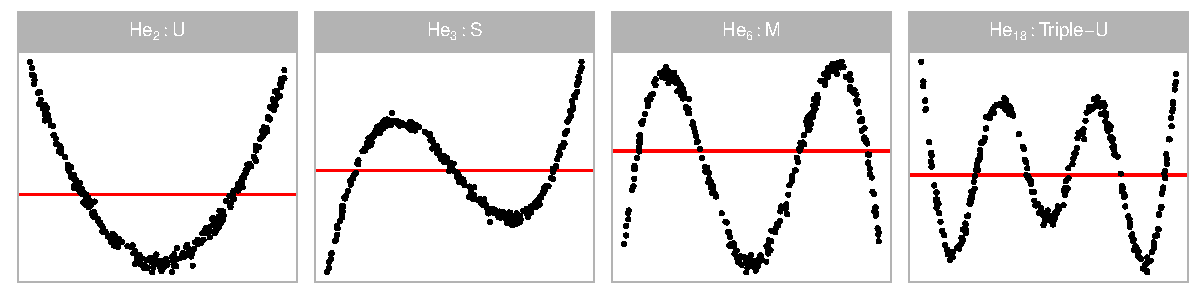
\includegraphics[width=1\linewidth]{paper_comparison_files/figure-latex/different-shape-of-herimite-1} \caption{Example residual plots of the linear regression model used in experiment I. Four different values of $j$ are included in the experiment results in four different shapes of residuals.}\label{fig:different-shape-of-herimite}
\end{figure}

Four different distribution were used to generate \(X_{raw}\) as shown
in Figure \ref{fig:different-dist}. The uniform and the normal
distribution are symmetric and commonly assumed in statistical models.
The adjusted log-normal distribution provides skewed density, while the
discrete uniform distribution provides discreteness in residual plot,
which could enrich the pool of visual patterns.

\begin{figure}
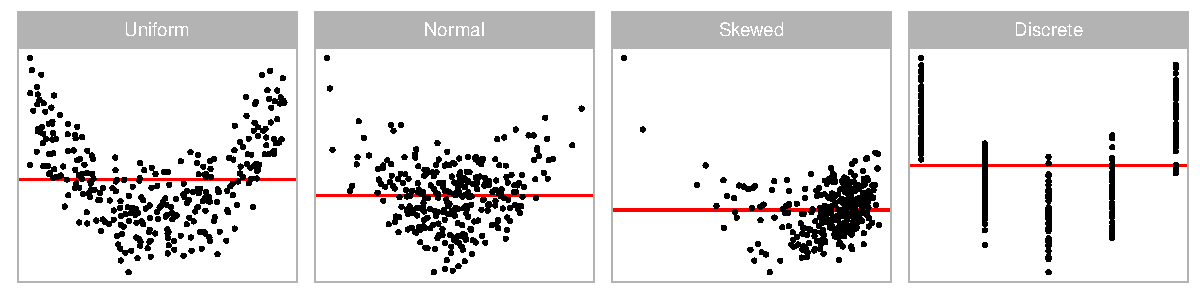
\includegraphics[width=1\linewidth]{paper_comparison_files/figure-latex/different-dist-1} \caption{Example residual plots of the linear regression model used in experiment I. Four different distribution of $x_{raw}$ are used in the experiment to provide various visual patterns.}\label{fig:different-dist}
\end{figure}

Figure \ref{fig:example-poly-lineup} shows one of the lineups used in
experiment I. This lineup was produced under \(j = 6\) and
\(X_{raw} \sim N(0.0.3^2)\). The actual data plot location was four. All
five subjects correctly identified the actual data plot for this lineup.

\begin{figure}
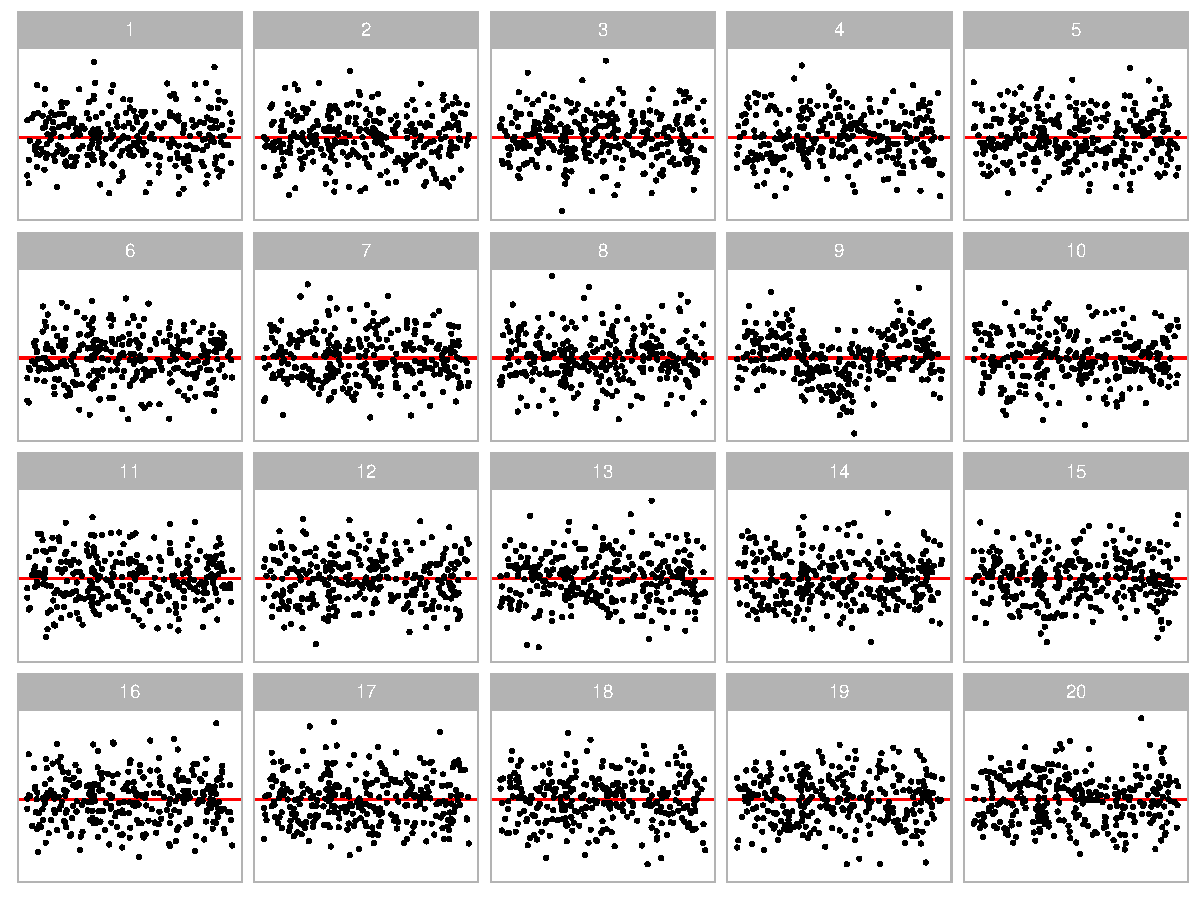
\includegraphics[width=1\linewidth]{paper_comparison_files/figure-latex/example-poly-lineup-1} \caption{Lineup poly-24 in experiment I. Can you spot the most different plot? \label{fig:example-poly-lineup}}\label{fig:example-poly-lineup}
\end{figure}

\hypertarget{heteroskedasticity}{%
\subsubsection{Heteroskedasticity}\label{heteroskedasticity}}

Experiment II is designed to study the ability of human subjects to
detect the appearance of a heteroskedasticity pattern under a simple
linear regression model setting:

\begin{align} \label{eq:heter-model}
\boldsymbol{y} = 1 + \boldsymbol{x} + \boldsymbol{\varepsilon},\\
\boldsymbol{x} = g(\boldsymbol{x}_{raw}, 1)\\
\boldsymbol{\varepsilon} \sim N(\boldsymbol{0}, 1 + 2 - |a| b (\boldsymbol{x} - a)^2 \boldsymbol{I}), \\
\end{align}

where \(\boldsymbol{y}\), \(\boldsymbol{x}\),
\(\boldsymbol{\varepsilon}\) are vectors of size \(n\) and \(g(.)\) is
the scaling function defined in \ref{eq:scaling-function}.

The null regression model used to fit the realizations generated by the
above model is formulated exactly the same as Equation
\ref{eq:null-model}.

For \(b \neq 0\), the variance-covariance matrix of the error term
\(\boldsymbol{\varepsilon}\) is correlated with the regressor \(x\),
which will lead to the presence of heteroskedasticity. Visual patterns
were simulated using three different shapes (\(a\) = -1, 0, 1) and the
same four different distribution of \(X_{raw}\) used in experiment I.

The values of \(a\) was chosen so that different shapes of
heteroskedasticity were included in the residual plot. These include
left-triangle shape, butterfly shape and right-triangle shape as
displayed in Figure \ref{fig:different-shape-of-heter}.

\begin{figure}
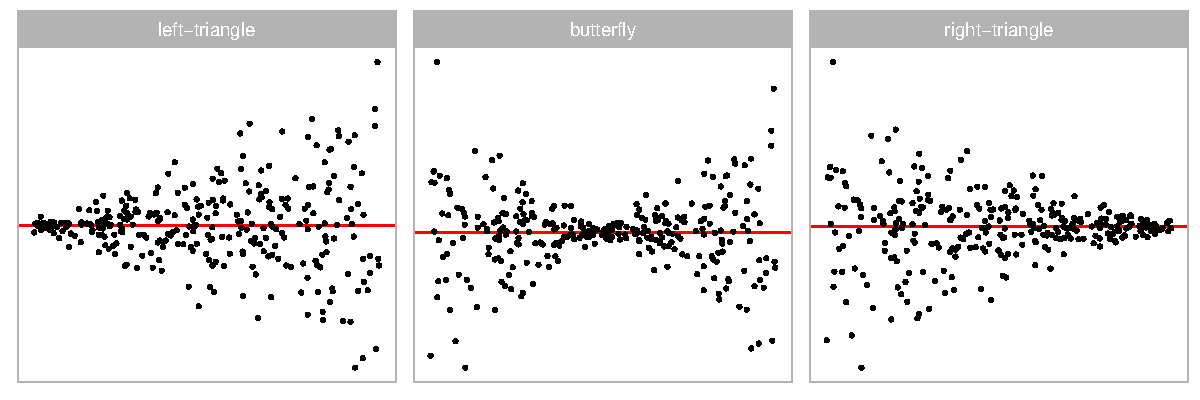
\includegraphics[width=1\linewidth]{paper_comparison_files/figure-latex/different-shape-of-heter-1} \caption{Example residual plots of the linear regression model used in experiment II. Three different shapes (a = -1, 0, 1) are used in the experiment to create left-triangle shape, butterfly shape and right-triangle shape.}\label{fig:different-shape-of-heter}
\end{figure}

\begin{figure}
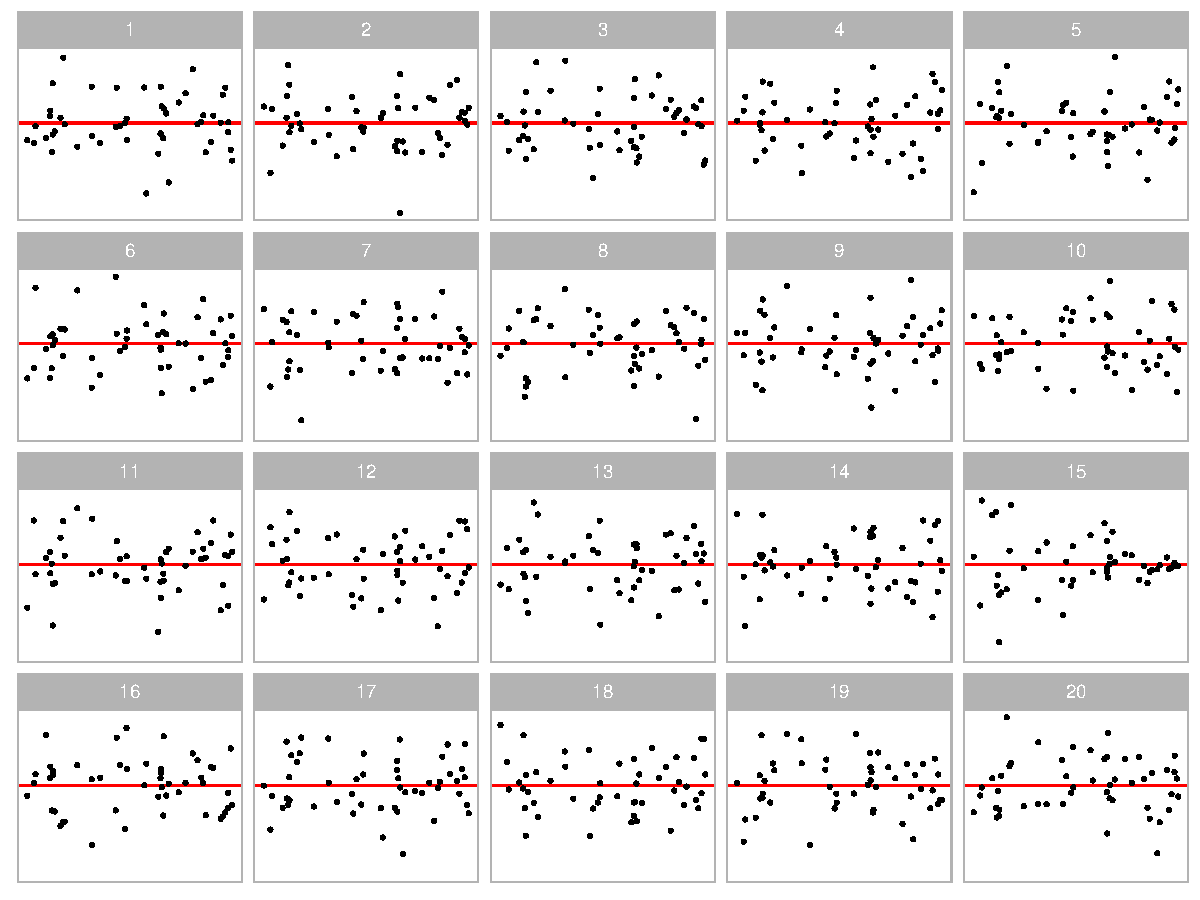
\includegraphics[width=1\linewidth]{paper_comparison_files/figure-latex/example-heter-lineup-1} \caption{Lineup heter-169 in experiment II. Can you spot the most different plot? \label{fig:example-heter-lineup}}\label{fig:example-heter-lineup}
\end{figure}

An example lineup of this model is shown in Figure
\ref{fig:example-heter-lineup} with \(a = -1\) and
\(X_{raw} \sim U(-1, 1)\). The actual data plot location was 15. 8 out
of 11 subjects correctly identified the actual data plot for this
lineup.

\hypertarget{experimental-setup}{%
\subsection{Experimental setup}\label{experimental-setup}}

\hypertarget{controlling-the-strength-of-the-signal}{%
\subsubsection{Controlling the strength of the
signal}\label{controlling-the-strength-of-the-signal}}

As summarised by Table \ref{tab:model-parameter-table}, three additional
parameters \(n\), \(\sigma\) and \(b\) were used to control the strength
of the signal so that different difficulty levels of lineups were
generated, and therefore, the estimated power curve would be smooth and
continuous. Parameter \(\sigma \in \{0.5, 1, 2, 4\}\) and
\(b \in \{0.25, 1, 4, 16, 64\}\) were used in experiment I and II
respectively. Figure \ref{fig:different-sigma} and \ref{fig:different-b}
demonstrate the impact of these two parameters.

Three different sample sizes were used (n = 50, 100, 300) in all three
experiments. It can be observed from Figure \ref{fig:different-n} that
with fewer data points drawn in a residual plot, the visual pattern is
more difficult to be detected.

\begin{figure}
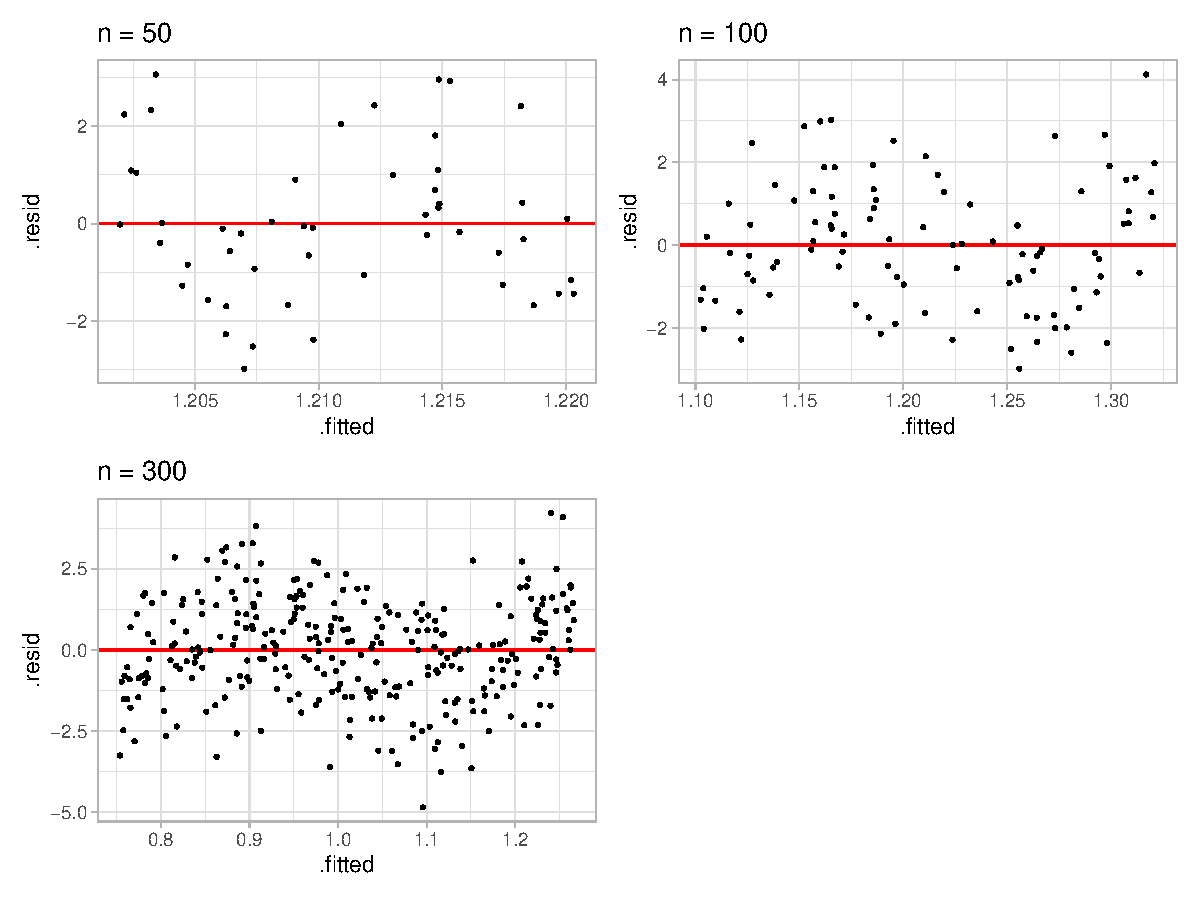
\includegraphics[width=1\linewidth]{paper_comparison_files/figure-latex/different-n-1} \caption{Three different values of $n$ are used in experiment I, II and III to control the strength of the signal.}\label{fig:different-n}
\end{figure}

\begin{figure}
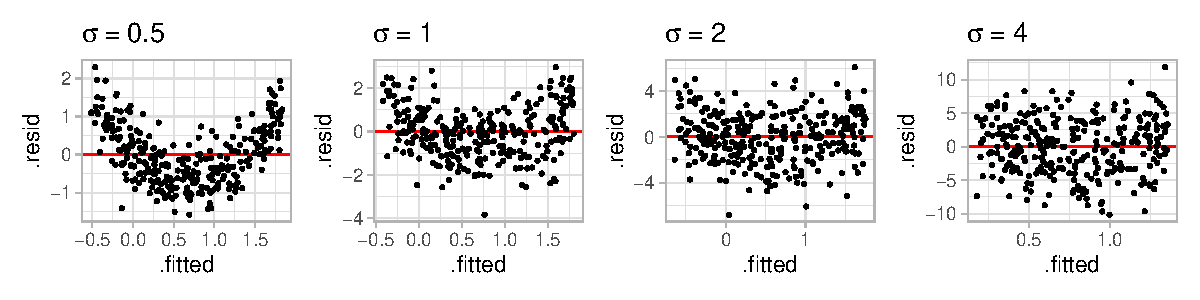
\includegraphics[width=1\linewidth]{paper_comparison_files/figure-latex/different-sigma-1} \caption{Example residual plots of the linear regression model used in experiment I. Four different values of $\sigma$ are included in the experiment to control the strength of the signal.}\label{fig:different-sigma}
\end{figure}

\begin{figure}
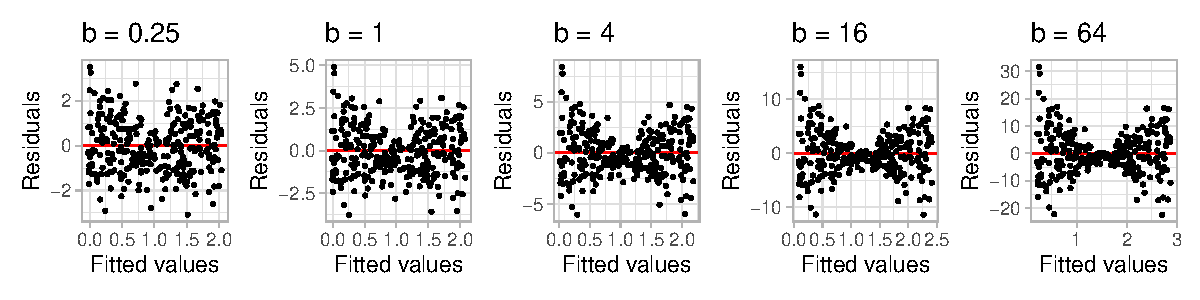
\includegraphics[width=1\linewidth]{paper_comparison_files/figure-latex/different-b-1} \caption{Example residual plots of the linear regression model used in experiment II. Five different values of $b$ are included in the experiment to control the strength of the signal.}\label{fig:different-b}
\end{figure}

\hypertarget{subject-allocation}{%
\subsubsection{Subject allocation}\label{subject-allocation}}

Three replications are made for each of the parameter values shown in
Table \ref{tab:parameter-table} resulting in 1152 different lineups. In
addition, each lineup is designed to be evaluated by five different
subjects and lineups with uniform distribution is designed to be
evaluated by 11 subjects to provide reasonable estimates of the visual
p-value.

Thus, \(443\) subjects were recruited to satisfy the design of the
experiment.

\hypertarget{collecting-results}{%
\subsubsection{Collecting results}\label{collecting-results}}

Subjects for all three experiments were recruited from an crowdsourcing
platform called Prolific {[}ref here{]}. Prescreening procedure was
applied during the recruitment, subjects were required to be fluent in
English, with \(98\%\) minimum approval rate in other studies and 10
minimum submissions. During the experiment, every subject was presented
with a block of 20 lineups. For each lineup, the actual data plot was
drawn as a standard residual plot of the null model with raw residuals
on the y-axis and fitted values on the x-axis. An additional horizontal
red line was added at \(y = 0\) as a helping line. The 19 null datasets
were generated by the residual rotation technique, and plotted in the
same way. The lineup consisted of 20 residual plots with one randomly
placed actual data plot. And for every lineup, the subject was asked to
select one or more plots that are most different from others, provide a
reason for their selections, and evaluate how different they think the
selected plots were from others. If there was no noticeable difference
between plots in a lineup, subjects were permitted to select zero plots
without providing the reason. No subject was shown the same lineup
twice. Information about preferred pronoun, age group, education, and
previous experience in visual experiment were also collected. In every
block of 20 lineups that presented to a subject, two lineups with
obvious visual patterns were included as attention checks. A subject's
submission was only accepted if the actual data plot was identified for
at least one attention check. Data of rejected submissions were
discarded automatically to maintain the overall data quality.

\hypertarget{results}{%
\section{Results}\label{results}}

\hypertarget{data-overview}{%
\subsection{Data overview}\label{data-overview}}

Subjects recruited from Prolific received a fixed payment for
participating in the experiment. However, some subjects will try to
maximize their earnings for minimum effort. During the review of
submissions, if we found a subject objectively demonstrated clear
low-effort throughout the experiment, i.e., failed all attention checks,
we rejected the submission. The rejected submissions will be removed
immediately, and Prolific will automatically recruit another subject as
substitution. Therefore, we only paid for approved submissions and no
further data screening procedure needed to be applied on the collected
data.

In overall, there were a total of 3200 lineup evaluations made by 160
subjects in both experiment I and experiment II respectively, where 320
lineup evaluations were attention checks and were not used in the
following analysis.

The collated dataset is provided in \texttt{vi\_survey} of the
\texttt{visage} \texttt{R} package.

\hypertarget{power-comparison}{%
\subsection{Power comparison}\label{power-comparison}}

Figure \ref{fig:power-poly-uniform} shows the estimated power of visual
test against natural logarithm of the effect with comparison to the
power of an exact test - F-test, and the power of two other
residual-based conventional tests commonly used in regression
diagnostics but for testing other departures from the model assumptions.
In overall, the power of all four tests increases as the effect becomes
larger. The power curve of F-test climbs aggressively from 25\% to
around 90\% as \(log_e(E)\) increases from 0 to 2, while others respond
inactively to the change of effect and remain lower than 25\% throughout
the period, showing that as an exact test, the F-test is relatively more
sensitive to the type of model defects that being considered. The power
of visual test arises steadily and nearly linearly to around 90\% as
\(log_e(E)\) increases from 2 to 5, suggesting that the effect starts to
make noticeable impact on the degree of the presence of the designed
visual features. Other two inappropriate conventional tests shows
improvement at the same time but at a lower rate. This coincides the
point made by \citet{cook1982residuals} mentioned in
\ref{hypothesis-testing} that residual-based tests for a specific type
of model defect are sensitive to other types of model defects. At
\(log_e(E) = 6\), the power curve of F-test reaches almost 100\%
followed by the visual test by a small margin. The power of
Breusch--Pagan test and Shapiro--Wilk test reach around 75\% and 30\%
respectively.

What truly impress us is the huge difference between the estimated power
of visual test and the estimated power of F-test. The margin is largest
at around \(log_e(E) = 2\). An example lineup is included in Figure
\ref{fig:power-overview} where none of subjects detect the actual data
plot positioned at panel 14. It demonstrates that at this level of
difficulty, the designed visual feature is rarely visible, making the
actual data plot indistinguishable from residual plots simulated from
the assumed model. From a communication perspective, given the fact that
the visual difference is unperceivable, the argument that non-linearity
present in the fitted model is less convincing to the public even though
it is true. At around \(log_e(E) = 3\), the margin gets smaller as the
chance of identifying the actual data plot becomes larger. At this level
of difficulty, the designed visual features are usually detectable but
it may not stand out from the lineup as other null plots may happen to
include outliers or visual patterns that are are considered to be more
attractive by human, and thus recognized as the most different plot.
Without knowing the designed visual features beforehand, it is actually
hard to identify the actual data plot by pure image comparison. The
corresponding example lineup for \(log_e(E) = 3\) shown in Figure
\ref{fig:fig:power-poly-uniform} has the actual data plot positioned at
panel 20, where two out of five subjects detect it. It can be observed
that a M-shape is presented in plot 20, but the signal is not strong
enough to attract all five subjects, resulting in a visual p-value
sightly above the desired significance level \(\alpha = 0.05\). At
\(log_e(E) = 4\) and \(log_e(E) = 6\), the designed visual features
become much clear and attractive, leading to a high percentage of
rejection of the null hypothesis. Figure
\ref{fig:fig:power-poly-uniform} gives example lineups of such cases. It
is also interesting to observe that the power curve of visual test
behaves similarly to those inappropriate conventional tests until the
designed visual features really becomes visible.

\begin{figure}
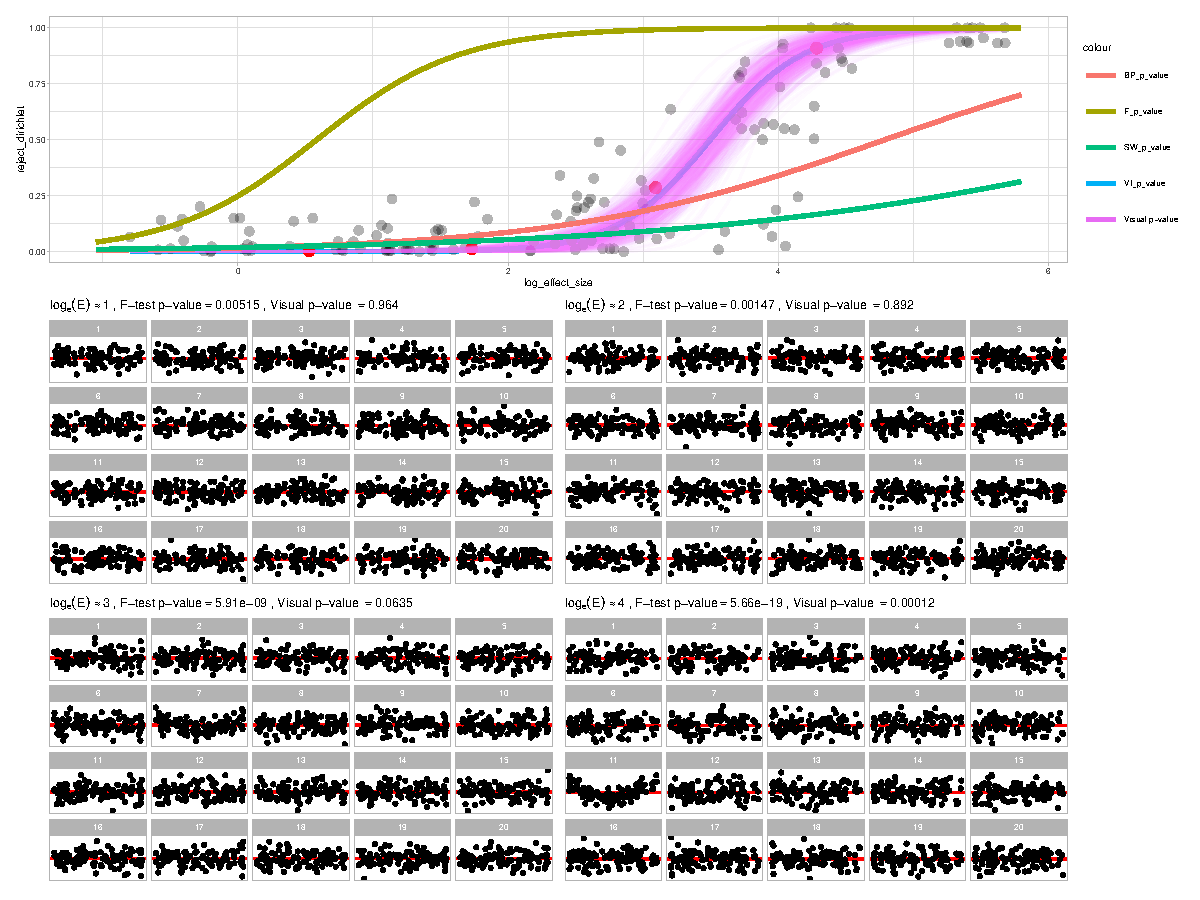
\includegraphics[width=1\linewidth]{paper_comparison_files/figure-latex/fig:power-poly-uniform-1} \caption{...}\label{fig:fig:power-poly-uniform-1}
\end{figure}
\begin{figure}
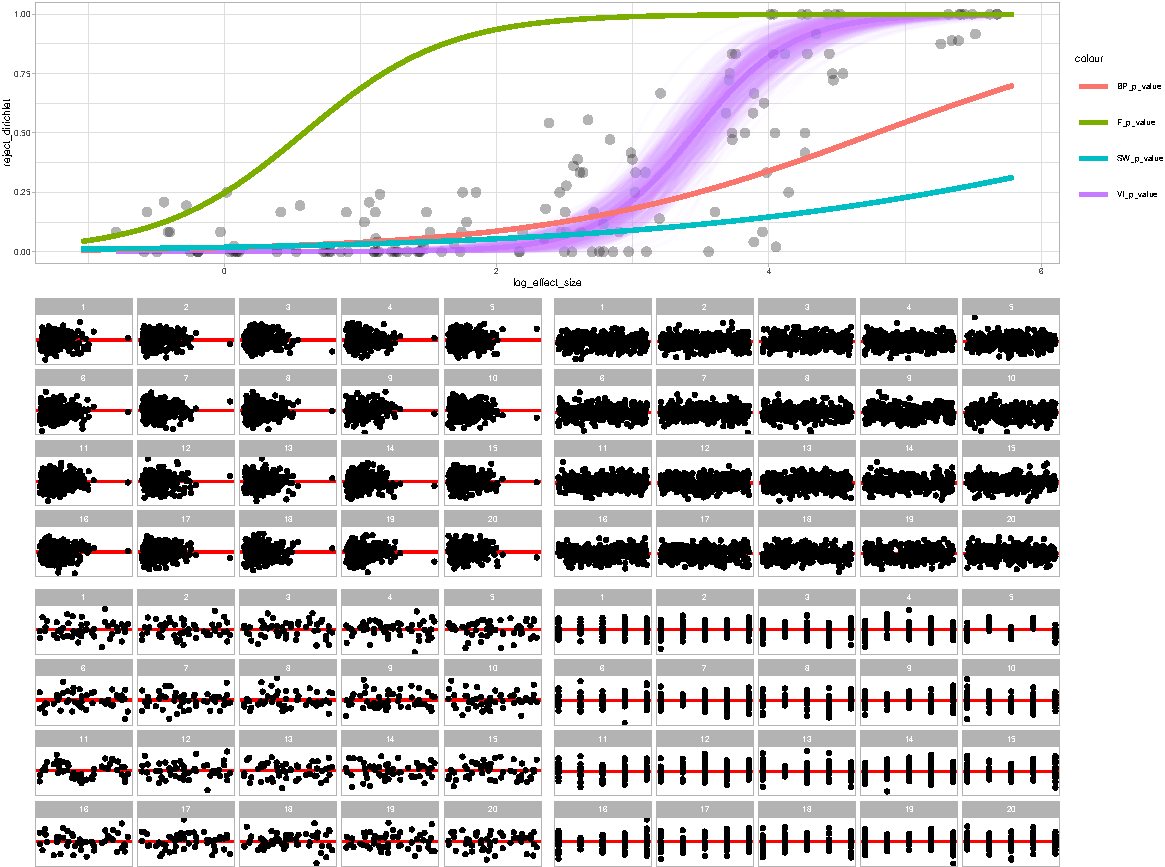
\includegraphics[width=1\linewidth]{paper_comparison_files/figure-latex/fig:power-poly-uniform-2} \caption{...}\label{fig:fig:power-poly-uniform-2}
\end{figure}

\hypertarget{distribution-of-regressor}{%
\subsection{Distribution of regressor}\label{distribution-of-regressor}}

The impact of the distribution of \(X_raw\) on the power is shown in
Figure \ref{fig:dist-power}. The power curve of F-test is stable across
different distributions, while the visual test has a steeper power curve
for normal and uniform distribution. BP-test performs worse for discrete
uniform distribution and uniform distribution but has relatively high
power for normal distribution. SW-test outperforms BP-test for discrete
uniform distribution but remains as the worst test for other
distributions. The results indicate those inappropriate residual-based
tests are sensitive to the distribution of the regressor.

\begin{figure}
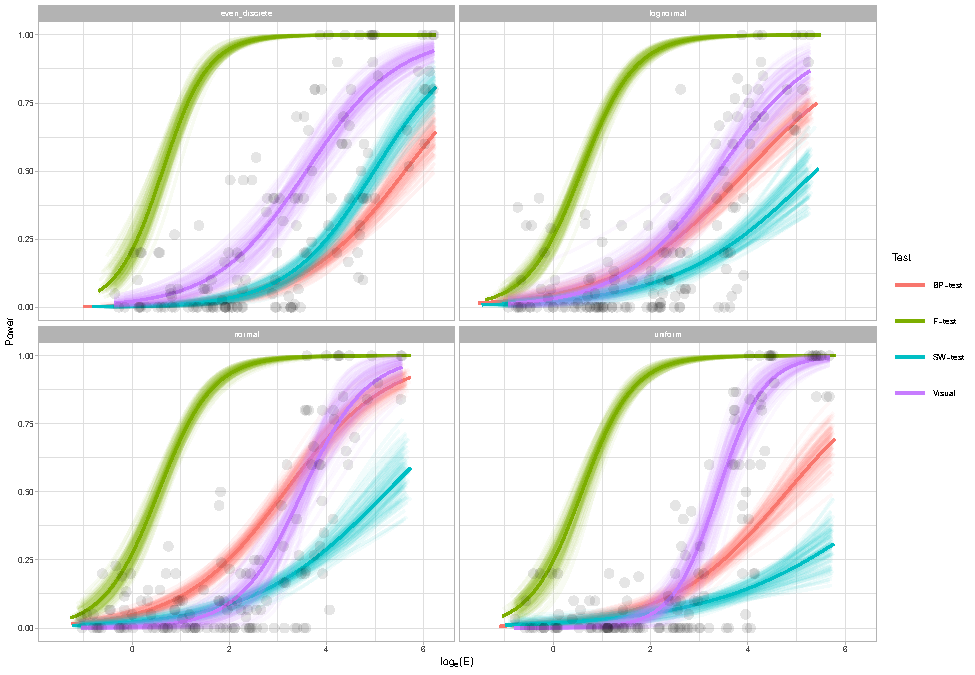
\includegraphics[width=1\linewidth]{paper_comparison_files/figure-latex/dist-power-1} \caption{...}\label{fig:dist-power}
\end{figure}

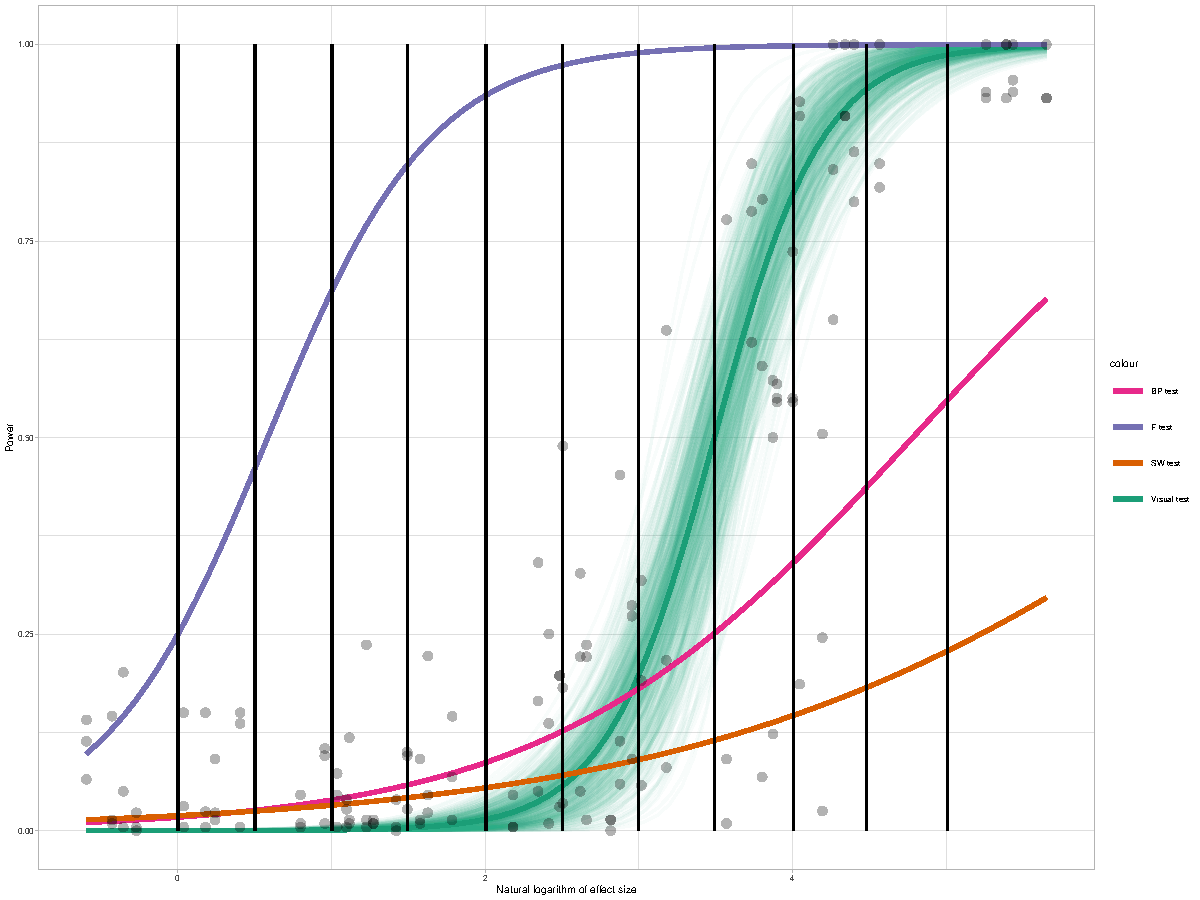
\includegraphics[width=1\linewidth]{paper_comparison_files/figure-latex/unnamed-chunk-6-1}

--\textgreater{}

--\textgreater{}

\bibliographystyle{tfcad}
\bibliography{paper.bib}




\end{document}
